\section{Tutorial: PintaFotos}

En este tutorial presentaremos el componente \component{Lienzo} para
crear aplicaciones con gráficos y animaciones simples en 2 dimensiones
(2D). Construirás la aplicación \appName{PintaFotos} que permite al
usuario dibujar en la pantalla usando distintos colores, usando una
imagen de fondo y dibujando sobre ella.

\emph{Un dato histórico}: PintaFotos fue uno de los primeros programas
desarrollados para demostrar el potencial de los computadores, en la
decada de 1970. En aquel entonces, hacer algo tan simple como esta
aplicación de dibujo era algo muy complejo, y los resultados no eran
perfectos. Pero ahora, con \AppInventor, cualquiera puede rápidamente
armar una aplicación de dibujo bastante buena, lo que sirve de
excelente punto de partida para luego hacer juegos 2D.

La interfaz de usuario de \appName{PintaFotos} se muestra en
la~\Cref{fig:appUI}.

\begin{figure}[H]
\centering
% 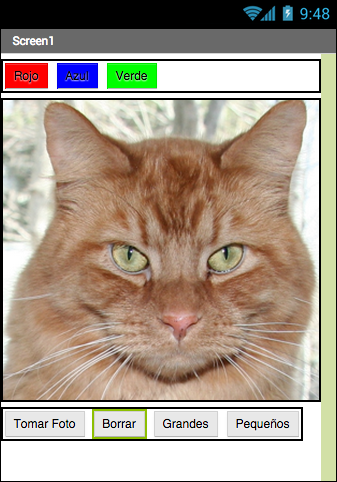
\includegraphics[scale=0.3]{PintaFotosUI}
\caption{Interfaz de usuario aplicación \appName{PintaFotos}}
\label{fig:appUI}
\end{figure}

En esta aplicación podrás:

\begin{itemize}
\item Bañar tu dedo en un tarro de pintura virtual para dibujar en
  este color.
\item Arrastrar tu dedo en la pantalla para dibujar una línea.
\item Tocar la pantalla para hacer puntos.
\item Usar el botón de abajo para limpiar la pantalla.
\item Agrandar o achicar el tamaño de los puntos con los botones
  abajo.
\item Sacar una foto con la cámara y luego dibujar encima de esta foto.
\end{itemize}

\subsection*{Qué Aprenderás}

Siguiendo este tutorial aprenderás a:

\begin{itemize}
\item Usar el componente \component{Lienzo} para dibujar.
\item Manejar las funcionalidades “touch” y “arrastrar” en la pantalla del equipo.
\item Configurar la disposición de los componentes en la pantalla.
\item Usar los controladores de eventos que reciben argumentos o
  parámetros.
\item Definir variables para recordar cosas como el tamaño de un punto
  elegido por el usuario para dibujar.
\end{itemize}

\subsection*{Para Empezar}

Aseguráte que tu computador y teléfono están configurados para usar
\AppInventor. Crea un nuevo proyecto y nombrálo \appName{PintaFotos}. Abre el
\blockEditor y comprueba que puedes probar tu aplicación en tu
dispositivo mediante la conexión USB. Consulta con tu tutor ante
cualquier problema!

Para empezar, ve al panel de propiedades a la derecha del \designer y
cambia el titulo de la pantalla a ``PintaFotos''. Deberías ver este
cambio reflejado en el teléfono, con el nuevo título apareciendo en la
barra de títulos de tu app.

Si estás preocupado por confundir el nombre de tu proyecto con el
nombre de la pantalla, no te preocupes! Hay tres nombres claves en
\AppInventor:

\begin{itemize}	

\item El nombre que eliges para tu proyecto mientras trabajes en
  él. También será el nombre de la aplicación cuando la quieras
  publicar. Nota que puedes hacer click en “Archivo” y seleccionar
  ``Guardar Como'' en el \designer para crear una nueva versión o
  cambiar el nombre de un proyecto.

\item El nombre de la componente, \component{Screen1}, que verás en el
  panel que contiene el listado de los componentes de la app. No
  puedes cambiar este nombre en esta versión de \AppInventor.

\item El título de la pantalla, él que ves en la barra de título del
  teléfono. Empieza siendo \component{Screen1}, que es el título que
  usaste en \appName{HolaGatito}. Pero lo puedes cambiar, como lo
  hicimos en \appName{PintaFotos}.
\end{itemize}

\subsection*{Diseñando los Componentes}

Para crear la app usarás los siguientes componentes:

\begin{itemize}

\item Tres componentes \component{Botón} para seleccionar pintura
  roja, azul o verde y un componente \component{DisposiciónHorizontal}
  para organizarlos.

\item Un componente \component{Botón} para limpiar el dibujo, y otros
  dos para cambiar el tamaño de los puntos.

\item Un componente \component{Lienzo}, que es la superficie para
  dibujar. El \component{Lienzo} tiene una propiedad
  \property{ImagenDeFondo}, que configuraremos como
  \mediafile{gatito.png} desde el tutorial \appName{Hola Gatito}. Más
  adelante, modificarás la app para que la imagen de fondo pueda ser
  una foto sacada por el usuario.

\end{itemize}

\subsubsection*{Crea los Botones de Colores}

Primero, crea los 3 botones de color usando las siguientes
instrucciones:

\begin{itemize}
\item Arrastra un \component{Botón} al \viewer y cambia su
  \property{Texto} a ``Rojo'', y su \property{ColorDeFondo} también a
  rojo.

\item En la lista de \componentList, selecciona el \component{Botón1}
  y presiona ``Cambiar Nombre'' para cambiar su nombre por
  \component{BotónRojo}. Observa que no se puede poner espacios en los
  nombres de los componentes, entonces es común poner en mayúscula la
  primera letra de cada palabra en el nombre.

\item De la misma manera, crea dos botones adicionales para azul y
  verde, nombrados \component{BotónAzul} y \component{BotónVerde}
  respectivamente. Ponlos debajo del botón rojo. Chequea tu trabajo
  comparándo con~\Cref{fig:paintPot1}.
\end{itemize}

\begin{figure}[H]
\centering
% 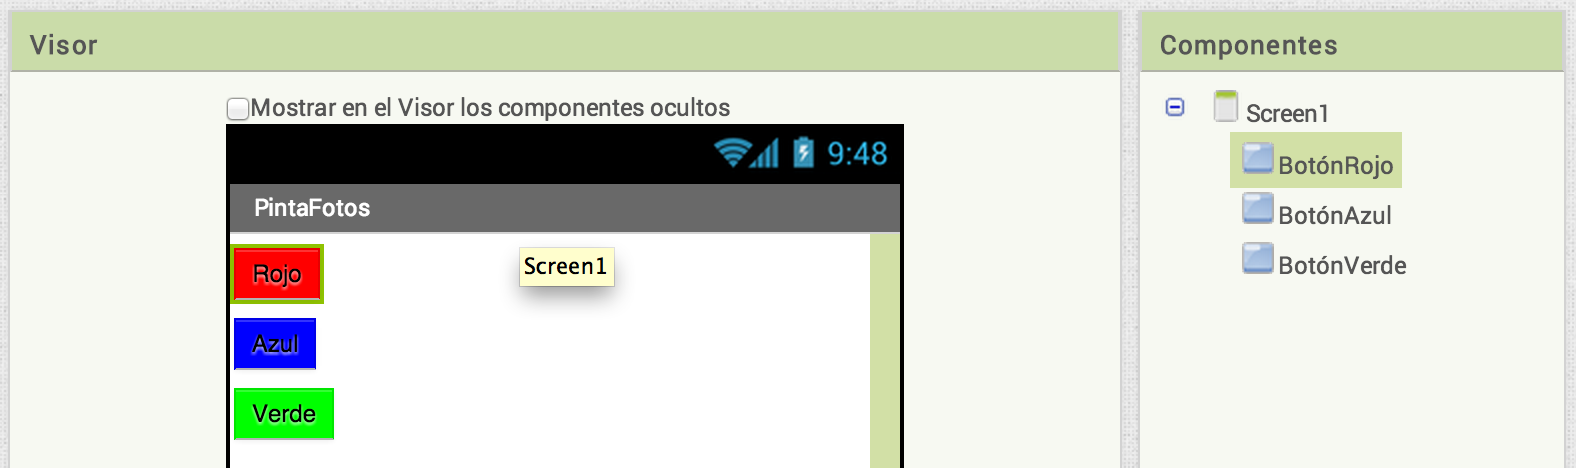
\includegraphics[scale=0.3]{PaintPot1}
\caption{El \viewer con los tres botones creados.}
\label{fig:paintPot1}
\end{figure}

\paragraph{Importante!}
Observa que en este proyecto cambias los nombres de los componentes en
vez de dejarlos con sus nombres por defecto, como lo hiciste en
\appName{Hola Gatito}. El usar nombres más significativos hace que tus
proyectos sean más fáciles de leer, y realmente ayuda en el momento de
pasar al \blockEditor cuando tendrás que referirte a los componentes
por su nombre. A partir de ahora y en el resto del taller usaremos la
convención de que cada nombre de componente empiece por su tipo (por
ejemplo: \component{BotónRojo}).

\paragraph{Prueba tu aplicación!} Conecta tu aplicación a tu
dispositivo y verifica que funcione correctamente.

\subsubsection*{Usando los Componentes de Disposición para una Mejor
  Presentación}

Ahora deberías tener tres botones alineados verticalmente. Sin embargo
para esta app, vas a necesitar que estén en fila horizontal arriba de
la pantalla, como en la~\Cref{fig:PaintPot2}. Para ello debes usar el
componente \component{DisposiciónHorizontal}.

\begin{figure}[H]
\centering
% 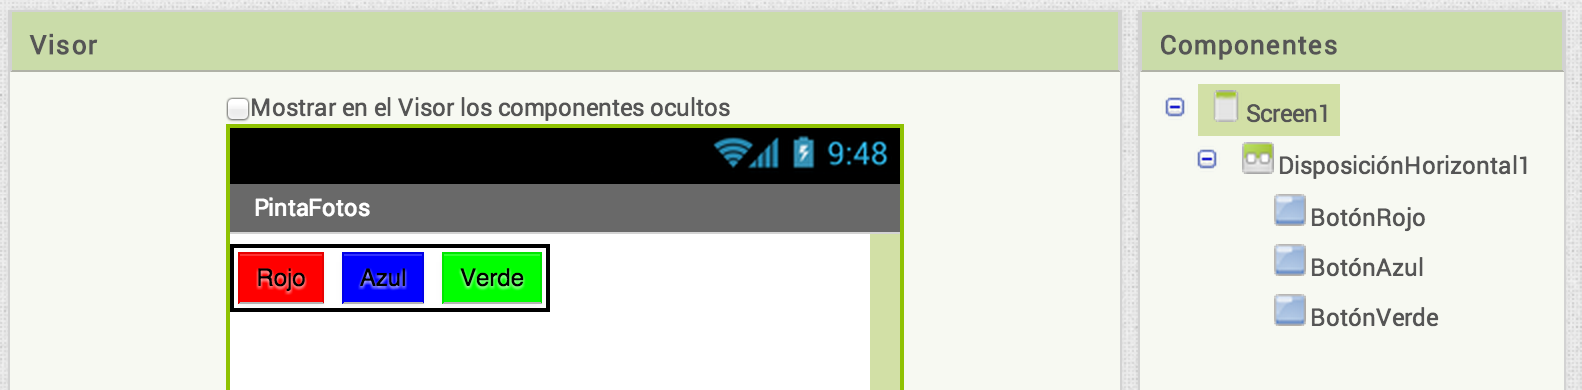
\includegraphics[scale=0.3]{PaintPot2}
\caption{Los tres botones en disposición horizontal.}
\label{fig:paintPot2}
\end{figure}

\begin{enumerate}

\item Desde la categoría “Disposición'' en la \palette, arrastra un
  componente \component{DisposiciónHorizontal} y ponlo debajo de los
  botones.

\item En el panel de \properties, cambia el \property{Ancho} de
  \component{DisposiciónHorizontal} a la opción ``Ajustar al
  contenedor'' para llenar todo lo ancho de la pantalla.

\item Mueve los tres botones uno después del otro al interior de la
  \component{DisposiciónHorizontal}. \emph{Truco}: Verás una línea
  vertical azul que indica dónde irá el elemento que estás
  arrastrando.

\end{enumerate}

Si miras en la lista de componentes del proyecto, verás tres botones
listados bajo el componente \component{DisposiciónHorizontal}, lo que
muestra que se trata de sus subcomponentes. Asímismo, observa que
todos los componentes están listados bajo el componente
\component{Screen1}.

\paragraph{Prueba tu Aplicación!} Deberías ver tus tres botones en una
fila horizonal en la pantalla, a pesar de que puedan verse un poco
diferente a como se ven en el \designer. Por ejemplo, el borde de
\component{DisposiciónHorizontal} no aparece en el dispositivo.

En general, se usan los componentes de ``Disposición'' como opciones
de diseño para crear disposiciones simples, verticales, horizontales o
en tablas. También puedes crear disposiciones más complejas insertando
componentes de disposición unos dentro de otros.

\subsubsection*{Agregar el Lienzo}

\begin{itemize}

\item El lienzo es el lugar donde el usuario dibuja círculos y
  líneas. Agregalo, y configura el archivo \mediafile{gatito.png},
  usado en \appName{Hola Gatito}, como su \property{ImagenDeFondo}.

\item Desde la categoría ``Dibujo y Animación'' de la \palette,
  arrastra un \component{Lienzo} hacia el \viewer. Cambia su nombre a
  \component{LienzoDeDibujo}. Configura su \property{Ancho} como
  ``Ajustar al Contenedor'' y su \property{Alto} a 300 pixeles.

\item Recuerda que puedes descargar el archivo \mediafile{gatito.png}
  desde \resources{ProgramaTusIdeas/Dia1/HolaGatito}.

\item Configura la \property{ImagenDeFondo} del
  \component{LienzoDeDibujo} con el archivo \mediafile{gatito.png}. Si
  es necesario, debes subir el archivo.

\item Cambia el \property{ColorDePintura} en el
  \component{LienzoDeDibujo} al color rojo para que cuando
  el usuario inicie la app pero todavía no ha presionado ningun botón,
  sus dibujos sean rojos. Comprueba si lo que has hecho es parecido a
  la~\Cref{fig:PaintPot3}.

\begin{figure}[H]
\centering
% 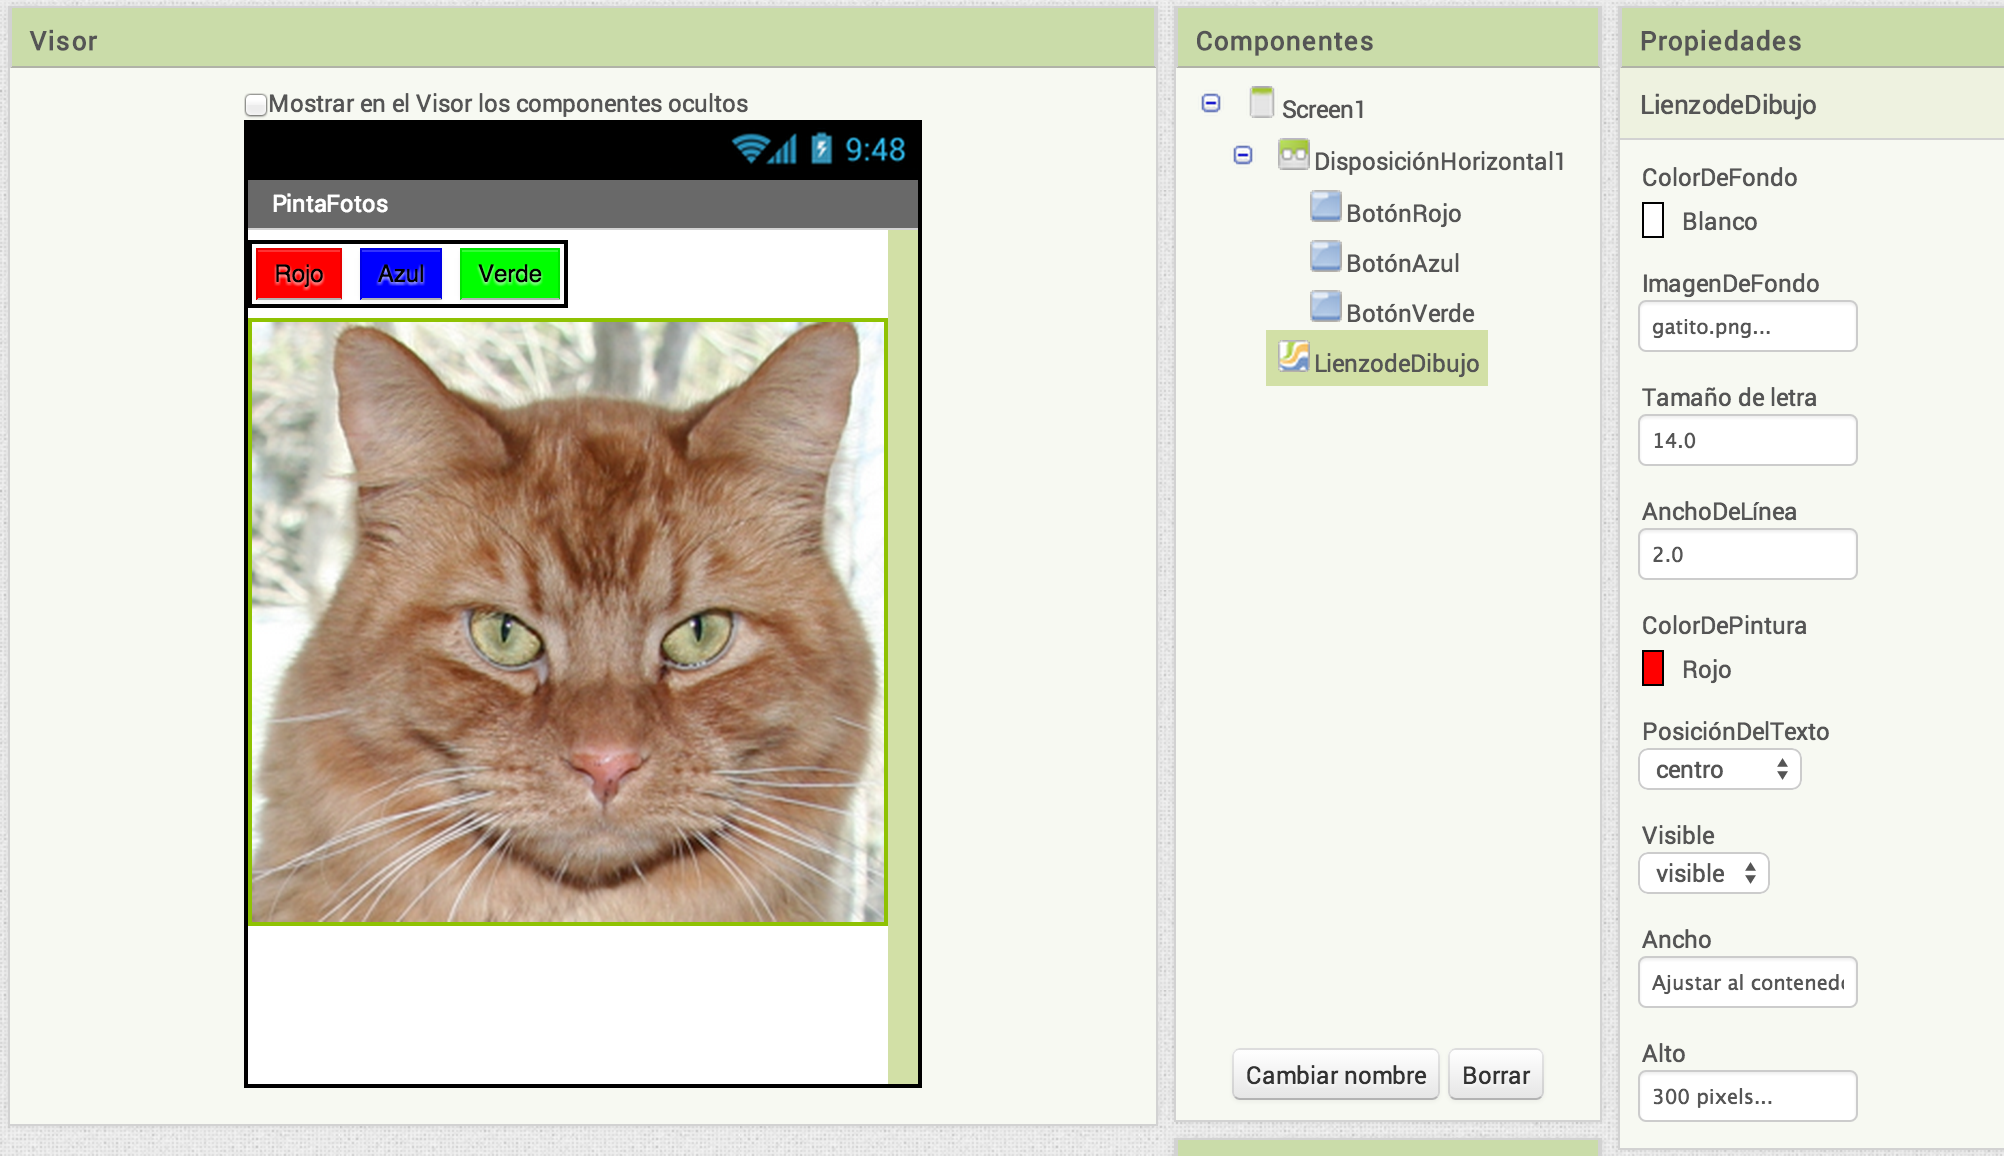
\includegraphics[scale=0.3]{PaintPot3}
\caption{El \component{LienzoDeDibujo} con la imagen
  \mediafile{gatito.png} como \property{ImagenDeFondo}.}
\label{fig:PaintPot3}
\end{figure}

\end{itemize}

\subsubsection*{Agregar los Botones Inferiores y el Componente Cámara}

\begin{enumerate}

\item Desde la \palette, arrastra un nuevo componente
  \component{DisposiciónHorizontal} y ponlo abajo del lienzo.

\item Luego arrastra dos componentes \component{Botón} adicionales en
  el \viewer y ponlos dentro del \component{DisposiciónHorizontal} que
  acabas de agregar. Cambia el nombre del primer botón por
  \component{BotonCámara} y su \property{Texto} a ``Sacar
  Foto''. Cambia el nombre del segundo botón por
  \component{BotonLimpiar} y su \property{Texto} por ``Limpiar''.

\item Arrastra dos botones más y colócalos al lado derecho del
  \component{BotónLimpiar}.

\item Nombra los nuevos botones como \component{BotónGrande} y
  \component{BotónPequeño}, y pon su \property{Texto} como
  ``PuntosGrandes'' y ``PuntosPequeños'' respectivamente.

\item Desde la sección \media de la \palette, arrastra un componente
  \component{Cámara} hacia el \viewer. Aparecerá en la sección de los
  componentes no-visibles.

\end{enumerate}
	
Una vez completados estos pasos, tu aplicación debería verse como en
la~\Cref{fig:PaintPot4}.

\begin{figure}[H]
\centering
% 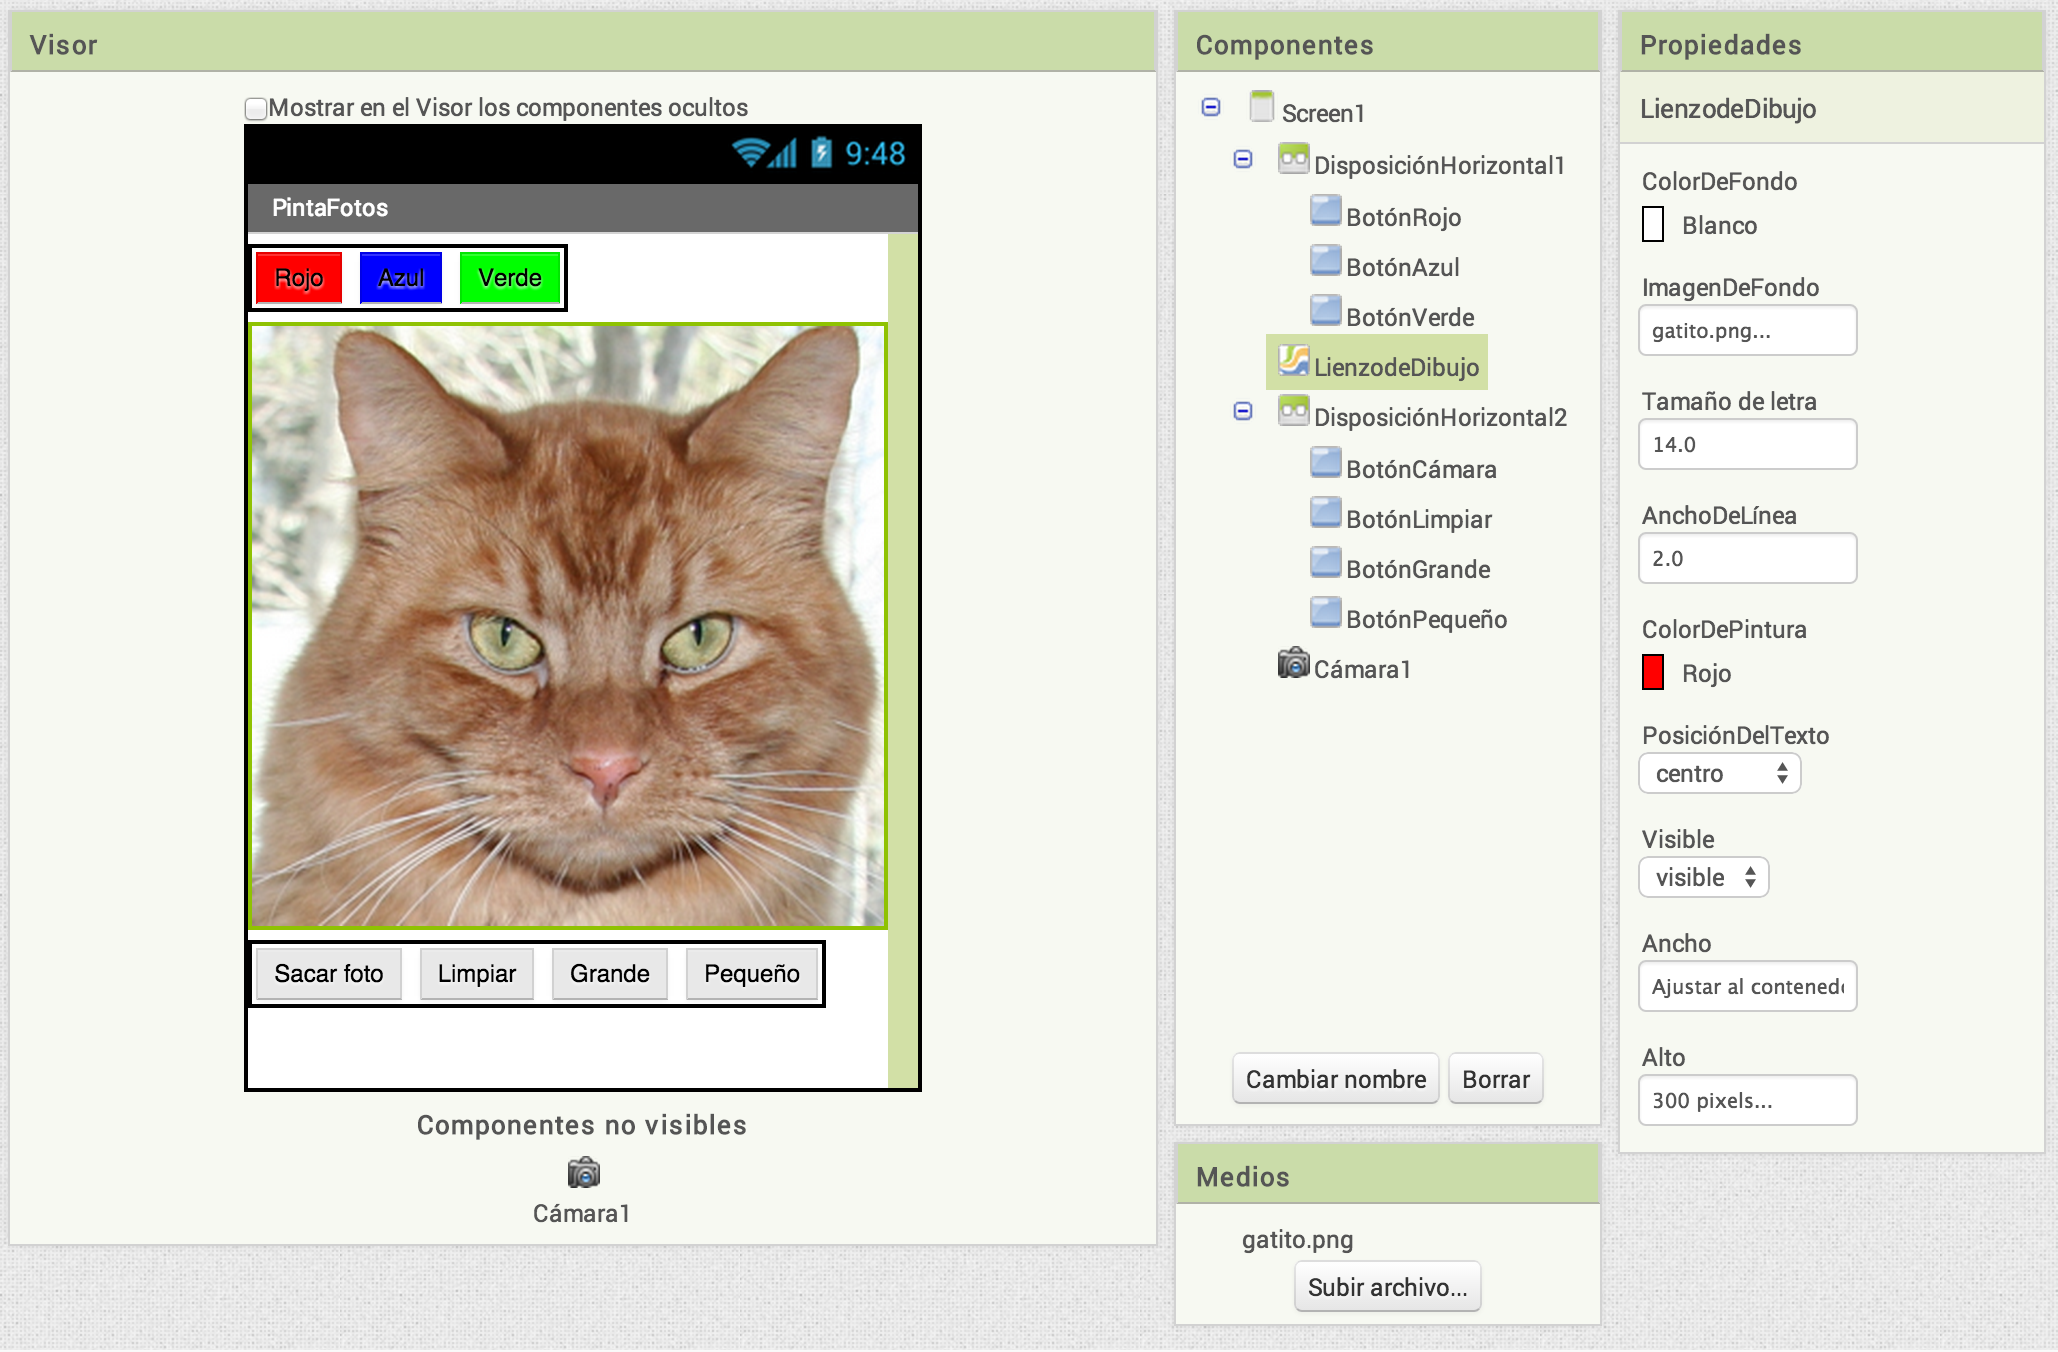
\includegraphics[scale=0.3]{PaintPot4}
\caption{Interfaz de usuario completa para \appName{PintaFotos}}
\label{fig:PaintPot4}
\end{figure}

\paragraph{Prueba tu Aplicación!} ¿Aparece la foto del gatito debajo
de los botones de la primera fila? ¿Aparece la última fila de botones abajo?

\subsubsection*{Agregar Comportamiento a los Componentes}

El próximo paso es definir cómo se comportan los componentes. Crear un
programa de pintura puede parecer un desafío insuperable, pero quedate
tranquilo! \AppInventor te facilita el trabajo: existen bloques muy
fáciles de usar para manejar las funcionalidades de touch y arrastre,
y para dibujar y sacar fotos.

En el \designer, agregaste un componente \component{Lienzo} llamado
\component{LienzoDeDibujo}. Como todos los componentes de ese tipo,
\component{LienzoDeDibujo} tiene un evento \block{Tocar} y un evento
\block{Arrastrado}. Programarás el evento \block{LienzoDibujo.Tocar}
de tal manera que llame a la función
\block{LienzoDibujo.DibujarCírculo}. Programarás el evento
\block{LienzoDibujo.Arrastrado} de tal manera que llame a la función
\block{LienzoDibujo.DibujarLínea}. Programarás luego los botones para
configurar la propiedad \property{ColorDePintura} usando el bloque
\block{poner LienzoDibujo.ColorPintura}, y para limpiar el
\component{LienzoDeDibujo}; y finalmente, programarás como cambiar la
\property{ImagenDeFondo} del lienzo por una foto sacada con la cámara
del dispositivo.

\section{Discusión y Ejercicios de Personalización}

\section{Tutorial: Atrapa el Topo}

\section{Proyecto}

\section{Material de Apoyo}

\subsection*{Componente Lienzo}

\subsection*{Variables}

\subsection*{Temporizadores}

\begin{figure}[H]
\centering
% 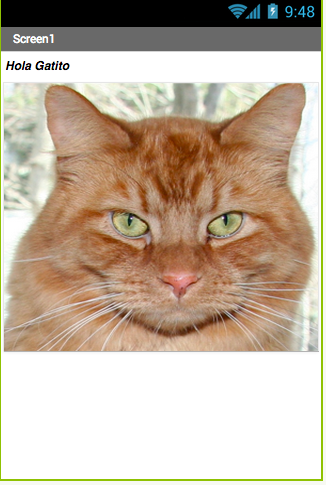
\includegraphics[scale=0.3]{HolaGatito}
\caption{Pantalla de aplicación \appName{Hola Gatito}}
\label{fig:holaGatito}
\end{figure}




\end{document}
